\section*{Zielsetzung}
\label{sec:Zielsetzung}
In diesem Versuch sollen verschiedene Emissions- und Absorptionsspektren untersucht
werden.

\section{Theorie}
\label{sec:Theorie}
\subsection{Erzeugung von Röntgenstrahlung}
\label{sec:Erzeugung von Röntgenstrahlung}
Für die Erzeugung von Röntgenstrahlung wird eine Röntgenröhre benutzt, ein evakuierter
Glaskolben mit einer Elektronen emitierenden Glühkathode und einer Anode. Wegen einer
elektrischen Spannung $U$ zwischen Kathode und Anode werden die Elektronen in Richtung Anode
beschleunigt. Trifft ein Elektron auf die Anode, so wird es abgebremst und emittiert seine
Energie in Form eines Photons. Da das Elektron nicht eine bestimmte Energie abgeben muss,
entsteht ein kontinuierliches Spektrum. Die maximale Energie bzw. die minimale Wellenlänge
eines Bremsphotons folgt aus dem Fall, dass die gesamte Potentialdifferenz $E = e_0 U$ in
Photonenenergie $E = h\nu$ umgesetzt wird. Gleichsetzen liefert die minimale Wellenlänge
\begin{equation}
	\label{eqn:lambda_min}
	\lambda_\text{min} = \frac{hc}{e_0 U}.
\end{equation}
% ionisierung und Leerstellen in der Anode
Eine alternative Erzeugung folgt aus Ionisierungen in der Anode. Dabei werden innere
Elektronenschalen frei und Elektronen aus höheren Energieniveaus können diese
``auffüllen``, wobei die Energiedifferenz $h\nu = E_m - E_n$ als Röntgenquant
ausgesendet wird. Wegen den diskreten Energieniveaus im Atom sind auch die
Energieübergänge diskretisiert, wodurch das Spektrum nicht mehr kontinuierlich ist,
sondern aus Emissionslinien besteht. Die Linien werden mit $K_\alpha, K_\beta, L_\alpha,
\hdots$ bezeichnet. Der lateinische Buchstabe bezeichnet die Zielschale des Übergangs, der
Griechische das Ursprungsniveau. 
\\
Weil bei größeren Atomen die inneren Elektronen den Kern abschirmen, wird die Coulomb
Anziehung durch den Kern verringert. Für das äußere Elektron folgt dann
\begin{equation}
	E_n = - R_\infty z_\text{eff}^2 \cdot \frac{1}{n^2}
\label{eqn:en}
\end{equation}
mit der effektiven Kernladung $z_\text{eff} = z - \sigma$, die die Abschirmung der
Elektronen in der Abschirmkonstante $\sigma$ beachtet. Bei der $K_\alpha$-Linie folgt dann
die Energie
\begin{equation}
	\label{eqn:eal}
	E_{K_\alpha} = R_\infty (z - \sigma_1)^2 \frac{1}{1^2} - R_\infty (z - \sigma_2)
	\frac{1}{2^2}.
\end{equation}
Die äußeren Elektronen besitzen aufgrund von Bahndrehimpuls und Spin nicht exakt die
gleiche Bindungsenergie und erzeugen eine Feinstruktur (Aufteilung in eng beieinander
liegende Linien); diese ist mit der verwendeten Apparatur jedoch nicht auflösbar.
\\
Der Absorptionskoeffizient ist dabei von der Photonenenergie abhängig. Im Energiespektrum
unter $\SI{1}{MeV}$ sind Compton- und Photoeffekt die dominanten Prozesse. Grundsätzlich
nimmt der Absorptionskoeffizient mit zunehmender Photonenenergie ab, steigt aber
sprunghaft wenn die Photonenenergie die Bindungsenergie eines inneren Elektrons
übersteigt. Dadurch entstehen im Spekturm sogenannte Absorbtionskanten, deren Energie
$h\nu = E_n - E_\infty$ ziemlich genau der Bindungsenergie des Elektrons entsprechen.
Entsprechend der Schale werden die Unstetigkeiten K-, L-, $\hdots$ Absorptionskanten
bezeichnet.

\subsection{Bragg`sche Bedingung}
\label{sec:Bragg`sche Bedingung}
\begin{wrapfigure}{r}{5cm}
	\begin{center}
		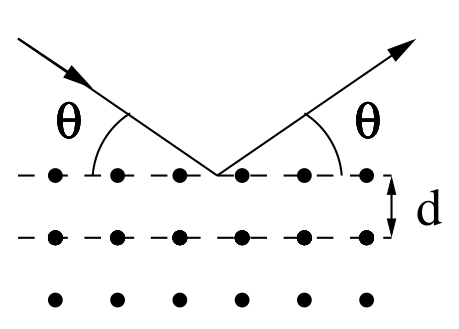
\includegraphics[width=5cm]{images/gitter.png}
	\caption{Ein Gitter mit Gitterkonstanten $d$ und Röntgenstrahl im Winkel
	$\theta$. \cite{V602}}
	\end{center}
	\label{fig:gitter}
\end{wrapfigure}
Für die experimentelle Bestimmung der Photonenergie bzw. der Wellenlänge $\lambda$ wird
die Bragg`sche Reflexion verwendet. Fällt die Röntgenstrahlung auf ein
dreidimensionales Gitter, z.B. auf einen Lithiumflouridkristall, werden die Photonen
gebeugt. Aus dem Gangunterschied folgt Interferenz; den Fall konstruktiver Interferenz
bezeichnet man mit dem Glanzwinkel $\theta$. Mit der Gitterkonstanten $d$ lässt sich die
Bragg`sche Bedingung
\begin{equation}
	2d \sin\theta = n\lambda
	\label{eqn:braggsche-bedingung}
\end{equation}
mit der Beugungsordnung $n$ herleiten. $d$ ist offensichtlich Materialabhängig, für den
verwendeten LiF-Kristall gilt $d_\text{LiF} = \SI{201.4}{\pm}$.

